\documentclass{beamer}

\mode<presentation>
{
  \usetheme{CambridgeUS}
  \setbeamercovered{transparent}
}

\usepackage[T1]{fontenc}
\usepackage[utf8]{inputenc}
\usepackage[spanish]{babel}
\usepackage{color}
\usepackage{hyperref}
\usepackage{algorithm,algorithmic}
\usepackage{colortbl}
\usepackage{graphicx}
\usepackage{minted}
\usepackage{multicol}

\usepackage[skins,minted]{tcolorbox}

\setminted[java]{
  linenos=true,
  fontfamily=tt,
  fontsize=\small,
  frame=leftline
}

\newminted[jsmall]{java}{
  fontsize=\footnotesize
  , linenos = false
  , frame=single
  , autogobble=true
}

\newtcblisting{java}[2][]{
  minted language=java,
  enhanced, listing engine=minted,
  listing only, #1, title=#2, left=2em
}

\setminted[bash]{
  linenos=true,
  fontfamily=tt,
  fontsize=\small,
  frame=leftline
}

\newtcblisting{bash}[2][]{minted language=bash,
  enhanced, listing engine=minted,
  listing only, #1, title=#2, left=2em
}

\usepackage{enumitem}
\setitemize{itemsep=1.2em,%
  label=\usebeamerfont*{itemize item}%
        \usebeamercolor[fg]{itemize item}%
        \usebeamertemplate{itemize item}
}

\title[\textbf{Programación 2}]{\textbf{Programación 2}}
\subtitle{Introducción al Lenguaje Java\\Elementos Básicos}
 
\author[IF-EG]
{
  Profesores:\\
  Ismael Figueroa -  \texttt{\small ifigueroap@gmail.com}\\
  \vspace{0.5mm}
  Eduardo Godoy - \texttt{\small eduardo.gl@gmail.com}
}

\institute[Universidad de Valparaíso]

\date{}

\begin{document}

\begin{frame}
  \titlepage
\end{frame}

% \begin{frame}
%   \frametitle{Contenido}
%   \tableofcontents%[pausesections]
% \end{frame}

\section{Java como Plataforma}

\subsection{Antecedentes Generales}

\begin{frame}
  \frametitle{Inicio de Java}

    \begin{itemize}
    \item \textbf{Desarrollado por:} Sun Microsystems en 1991.
    \item \textbf{Propietario actual:} Oracle Corporation desde 2010.
    \item \textbf{Objetivo inicial y actual:}
      
      \begin{itemize}
      \item Desarrollar un lenguaje de programación para crear
        software peque\~nos, rápidos, eficientes y portátiles para
        diversos dispositivos de hardware (teléfonos celulares,
        radiolocalizadores y asistentes digitales personales).
        
      \item Ser el nexo universal que conecte a los usuarios con la
        información que esté situada en el computador local, en un
        servidor Web o en una base de datos.
      \end{itemize}
      
    \item \textbf{Principio:} \emph{Write Once, Run Everywhere}
      
    \end{itemize}    

\end{frame}

\begin{frame}
  \frametitle{Independencia de la Plataforma}
  
    \begin{itemize}
    \item \textbf{Tanto a nivel del código fuente como del binario.}



      \item \emph{\bf Independencia en código fuente}: los tipos
        primitivos de datos de Java tienen tama\~no consistentes en
        todas las plataformas de desarrollo. Las bibliotecas de Java
        facilitan la escritura del código, que puede desplazar se
        plataforma a plataforma.

      \item \emph{\bf Independencia en binario}: los archivos binarios
        (bytecodes) pueden ejecutarse en distintas plataformas sin
        necesidad de volver a compilar la fuente.
        
        % \begin{itemize}
        %	\item bytecodes: conjunto de instrucciones maás abstracto que el código máquina (código intermedio), pero no son especificas a un procesador.
        % \end{itemize}
      
    \end{itemize}
  
\end{frame}

\begin{frame}
  \frametitle{Ventajas}
    \begin{itemize}
    \item Fomenta la reutilización y extensión del código.
    \item Permite crear sistemas más complejos.
    \item Relacionar el sistema al mundo real.
    \item Facilita la creación de programas visuales.
    \item Elimina redundancia a través de la herencia y polimorfismo
    \item Agiliza el desarrollo de software.
    \end{itemize}
\end{frame}

\begin{frame}
  \frametitle{Más Ventajas}  
    \begin{itemize}
    \item Facilita el trabajo en equipo.
    \item Facilita el mantenimiento del software.
    \item Recolección de basura.
    \item En Java no hay punteros (simplicidad).
    \item Las cadenas y los arreglos son objetos reales
    \item La administración de la memoria es automática
    \end{itemize}
\end{frame}

\subsection{Infraestructura de Desarrollo}  

\begin{frame}
  \frametitle{Proceso de Compilación, Interpretación y Ejecución}
  \begin{center}
    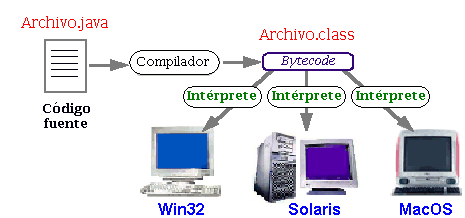
\includegraphics[scale=.65]{images/funcionamiento_java.png}
  \end{center}
\end{frame}  

\begin{frame}
  \frametitle{El Compilador {\texttt javac}}
  \framesubtitle{Ambiente de desarrollo Java}

  \begin{itemize}    
    \item Toma como entrada los archivos {\tt *.java} y configuraciones sobre el \emph{classpath}
    \item Genera archivos compilados en \emph{bytecode} en archivos {\tt *.class}      
    \item El \emph{classpath} indica dónde buscar otras clases
      externas a nuestro programa, tales como librerías
  \end{itemize}
\end{frame}

\begin{frame}
  \frametitle{La Máquina Virtual de Java --- JVM}

  Los archivos de bytecode son ejecutados por la JVM.

  \begin{itemize}
  \item La JVM carga el archivo de bytecode, y verifica qué este
    correctamente formado
    
  \item \textbf{Intérpretación inicial:} inicialmente el programa es
    ejecutado por el \emph{intérprete JVM}, que es una forma lenta de
    ejecutar, pero que puede partir de inmediato
    
  \item \textbf{Compilación Just-in-Time}: durante la ejecución, la
    JVM va progresivamente compilando al lenguaje máquina de la
    plataforma, para mejorar la velocidad de ejecución
    
  \end{itemize}
  
\end{frame}

\begin{frame}
  \frametitle{El Kit de Desarrollo --- JDK}

  \begin{exampleblock}{}
  Contiene las herramientas, programas, bibliotecas, y todos los
  elementos necesarios para el desarrollo y depuración de aplicaciones Java
  \end{exampleblock}

\end{frame}


\begin{frame}
  \frametitle{JDK / Compilación y Ejecución}  

  \begin{itemize}
    
  \item \texttt{javac}: es el compilador de Java, incluido solamente
    en el JDK. Se ejecuta desde línea de comandos: \texttt{javac HolaMundo.java}

  \item \texttt{java}: es el ejecutor de programas Java, se incluye
    tanto en el JDK como en el JRE. También se usa desde la línea de
    comandos: \texttt{javac HolaMundo.class}

  \item \texttt{javadoc}: Crea documentación en formato HTML a partir
    de el código fuente y los comentarios. Se usa desde la línea de
    comandos: \texttt{javadoc HolaMundo.java}    
    
  \end{itemize}

\end{frame}

\begin{frame}
  \frametitle{JDK / Utilitarios}

  \begin{itemize}
    
  \item \texttt{jar}: crea librerías en formato JAR (Java ARChive),
    que permite empaquetar clases y otros recursos en un único paquete
    portable

  \item \texttt{jdb}: depurador de Java, con soporte para breakpoints
    y avance paso a paso. Se usa sobre archivos bytecode: \texttt {jdb
      HolaMundo 10} (10 es la linea del breakpoint). \emph{En general
      no se usa manualmente sino como parte de un editor integrado}
        
  \end{itemize}

\end{frame}
 
\begin{frame}[fragile]
  \frametitle{Hola Mundo en Java}

  \begin{java}{HolaMundo.java}
    public class HolaMundo {
      public static void main(String[] args) {
        System.out.println("Hola Mundo!");
      }
    }
  \end{java}

\end{frame}

\begin{frame}[fragile]
  \frametitle{Ejecutando Hola Mundo}

  \begin{bash}{Compilación y ejecución usando {\tt javac} y {\tt java}}
    > javac HolaMundo.java
    > java HolaMundo
    Hola Mundo!
  \end{bash}

\end{frame}

\section{El Lenguaje de Programación Java}

\begin{frame}[fragile]
  \frametitle{La Clase Principal}  
  \begin{columns}
    \begin{column}{0.4\textwidth}
      \begin{itemize}
      \item Todo método debe necesariamente pertenecer a una
        clase.

      \item Todo programa ejecutable debe tener una \emph{clase
          principal}, que en general se llama {\tt Main}.

      \item La clase principal \textbf{debe} contener el método {\tt main}
    \end{itemize}
    \end{column}
    
    \begin{column}{0.6\textwidth}
      
      \begin{jsmall}
        public class Main {
          public static void main(String[] args) {
            /* codigo metodo principal */
          }
        }
      \end{jsmall}
      
    \end{column}
  \end{columns}
\end{frame}


\subsection{Tipos de Datos Primitivos}

\begin{frame}
  \frametitle{Tipos de Datos Primitivos}
  
  \begin{block}{}
    Se llaman \textbf{tipos primitivos} a aquellos que tienen los
    tipos de información más habituales: valores boolean, caracteres y
    valores numéricos enteros o de punto flotante. Son definidos por
    defecto en la JVM, y están soportados en todas las plataformas
    donde la JVM funcione.
  \end{block}
\end{frame}

\begin{frame}
  Java dispone de \textbf{ocho} tipos primitivos de variables:

  \begin{itemize}
  \item \texttt{boolean}: permite valores \texttt{true} y \texttt{false}
  \item \texttt{char}: representa characteres
  \item \texttt{byte, short, int, long}: valores enteros, de distintos
    tamaños máximos y mínimos    
  \item \texttt{float, double}: valores reales de punto flotante, con
    distinta precisión
  \end{itemize}

\end{frame}

\begin{frame}
  \frametitle{Precisión de los Tipos Primitivos} 

  {\small
    \begin{center}
      \begin{tabular}{|l|l|l|} \hline
        \multicolumn{1}{|>{\columncolor[rgb]{0.8, 0.8, 0.8}}l|}
        {\textbf{Tipo de variable}} & \multicolumn{1}{|>{\columncolor[rgb]{0.8, 0.8, 0.8}}l|}{\textbf{Descripción}} \\ \hline
        \texttt{boolean} & 1 byte. Valores \texttt{true} y \texttt{false} \\ \hline
        \texttt{char} 	 & 2 bytes. Unicode. Comprende el código ASCII \\ \hline
        \texttt{byte} 	 & 1 byte. Entero entre -128 y 127 \\ \hline
        \texttt{short} 	 & 2 bytes. Entero entre -32768 y 32767 \\ \hline
        \texttt{int}	 & 4 bytes. Entero entre -2.147.483.648 y
        \\               & 2.147.483.647. \\ \hline
        \texttt{long} 	 & 8 bytes. Valor entre -9.223.372.036.854.775.808 y
        \\               & 9.223.372.036.854.775.807. \\ \hline
        \texttt{float}	 & 4 bytes (entre 6 y 7 cifras decimales equivalentes). 
        \\ 	         & De -3.402823E38 a -1.401298E-45 y 
        \\		 & de 1.401298E-45 a 3.402823E38. \\ \hline
        \texttt{double}	 & 8 bytes (unas 15 cifras decimales equivalentes). 
        \\ 			 & De -1.79769313486232E308 a -4.94065645841247E-324
        \\ 			 & y de 4.94065645841247E-324 a 1.79769313486232E308. \\ \hline
      \end{tabular}
    \end{center}
  }
\end{frame}

\begin{frame}
  \frametitle{Características de los Tipos Primitivos}
  
  Los tipos primitivos de Java tienen algunas características importantes:

  \begin{itemize}
  \item El tipo \texttt{boolean} no es un valor numérico.

    \begin{itemize}
    \item Sólo admite los valores \texttt{true} o \texttt{false}. 
    \item El tipo boolean no se identifica con el igual o distinto de cero, como en otros lenguajes.
    \item El resultado de la expresión lógica para un \texttt{if} o
      similares \textbf{debe} ser de tipo booleano
    \end{itemize}
    
  \item El tipo \texttt{char} contiene caracteres en código Unicode
    (que incluye el código ASCII), y ocupan 16 bits (2 bytes) por
    carácter. Comprende los caracteres de prácticamente todos los
    idiomas.
  \end{itemize}
\end{frame}

\begin{frame}
  \frametitle{Características de los Tipos Primitivos}
  
  \begin{itemize}
  \item Los tipos \texttt{byte, short, int y long} son números enteros
    que pueden ser positivos o negativos, con distintos valores
    máximos y mínimos. A diferencia de otros lenguajes, en Java no hay
    enteros \texttt{unsigned}.
    
  \item Los tipos \texttt{float} y \texttt{double} son valores de
    punto flotante, números reales, con 6-7 y 15 cifras decimales
    exactas---significativas---respectivamente.
    
  \item Se utiliza la palabra \texttt{void} para indicar la ausencia
    de un tipo de variable determinado.
    
  \end{itemize}
\end{frame}

\begin{frame}
  \frametitle{Portabilidad de los Tipos Primitivos} 

  \begin{block}{}
    A diferencia de otros lenguajes, los tipos de variables en Java
    están perfectamente definidos en todas y cada una de las posibles
    plataformas soportadas por la JVM. Por ejemplo, un \texttt{int}
    ocupa siempre la misma memoria y tiene el mismo rango de valores,
    en cualquier plataforma soportada.
  \end{block}
\end{frame}

\subsection{Variables}

\begin{frame}
  \frametitle{Variables}

  \begin{block}{}
    Una variable es un nombre asociado a un valor en memoria. Las
    variables se llaman así porque el valor asociado puede cambiar
    durante la ejecución del programa.
  \end{block}

  \begin{block}{}
    En Java todas las variables están asociadas a un tipo de dato, sea
    este primitivo o de referencia.
  \end{block}

\end{frame}

\begin{frame}[fragile]
  \frametitle{Definición de Variables} 

  \begin{columns}
    \begin{column}{0.4\textwidth}
      \begin{small}
      \begin{itemize}
      \item Una variable se define especificando el tipo y el nombre
        de dicha variable
        
      \item Estas variables pueden ser tanto de tipos primitivos como
        referencias a objetos de alguna clase
        
      \item Las variables deben ser inicializadas antes de su uso, en
        otro caso tendrán valores nulos, y no podrán ser usadas
        
      \end{itemize}
      \end{small}
    \end{column}
    %
    \begin{column}{0.6\textwidth}
      \begin{jsmall}
        public class Auto {
          // Atributos marca y agno
          String marca;
          Integer agno;

          // Variable parametro km
          void acelerar(Integer km) {
            // Variable local aux
            int aux = 15;
            /* ... */
          }
        }        
      \end{jsmall}
    \end{column}
  \end{columns}
\end{frame}

\begin{frame}[fragile]
  \frametitle{Variables y Tipos de Referencia}

  \begin{columns}
    \begin{column}{0.4\textwidth}      
      Hay dos tipos de variables, según su tipo:
      \begin{itemize}
      \item De \textbf{tipos primitivos}: entero, float, etc.        
      \item De \textbf{referencia} u \textbf{objeto}: funcionan como
        referencias a objetos de cualquier clase.        
      \end{itemize}
      Esto cobra relevancia cuando se pasan como argumento a los métodos
    \end{column}
    %
    \begin{column}{0.6\textwidth}      
      \begin{jsmall}
        // Tipos primitivos
        int valor = 0;
        double = 3.14;

        // De referencia
        String nombre = "Juan";
        ArrayList a = new ArrayList();
      \end{jsmall}
    \end{column}
  \end{columns}  
\end{frame}  


\begin{frame}[fragile]
  \frametitle{Variables Locales y Como Atributos de Clase}

  \begin{columns}    
    \begin{column}{0.4\textwidth}
      \begin{small}
      \begin{itemize}
      \item \textbf{Atributos:} son variables que se definen en la
        clase, fuera de los métodos, y que definen las características
        propias de cada instancia.

        
      \item \textbf{Parámetros de métodos:} son aquellas que se
        reciben como parámetro de un método. \emph{Java siempre usa
          paso por valor!}
        
      \item \textbf{Variables locales de método:} son aquellas que se
        definen solo dentro de un método, para su adecuado
        funcionamiento
        
      \end{itemize}
      \end{small}
      
    \end{column}
    %
    \begin{column}{0.6\textwidth}
      \begin{jsmall}
        public class Auto {
          // Atributos marca y agno
          String marca;
          Integer agno;

          // Variable parametro km
          void acelerar(Integer km) {
            // Variable local aux
            int aux = 15;
            /* ... */
          }
        }        
      \end{jsmall}      
    \end{column}
  \end{columns}

\end{frame}

\begin{frame}
  \frametitle{Nombres de Variables}
    \begin{itemize}
    \item Los nombres de variables en Java se pueden crear con mucha
      libertad.
      
    \item Pueden ser cualquier conjunto de caracteres numéricos y
      alfanuméricos, sin algunos caracteres especiales utilizados por
      Java como operadores o separadores (\textbf{,.+-*/} etc).
      
    \item Existe una serie de palabras reservadas las cuales tienen un
      significado especial para Java y por lo tanto no se pueden
      utilizar como nombres de variables.
      
    \end{itemize}
\end{frame}

\begin{frame}
  \frametitle{Palabras Reservadas para Nombres}
  \begin{center}
    \begin{tabular}{|c|c|c|c|c|c|} \hline
      abstract    & boolean    & break     & byte         & case     & catch \\ \hline
      char        & class      & const     & continue     & default  & do    \\ \hline
      double      & else       & extends   & final        & finally  & float \\ \hline
      for         & goto       & if        & implements   & import   & instanceof \\ \hline
      int         & interface  & long      & native       & new      & null \\ \hline
      package     & private    & protected & public       & return   & short \\ \hline
      static      & super      & switch    & synchronized & this     & throw \\ \hline
      throws      & transient  & try       & void         & volatile & while \\ \hline
    \end{tabular}
  \end{center}
\end{frame}

\begin{frame}
  \frametitle{Variables de Referencia} 
  \begin{itemize}
  \item Las variables con tipo de referencia indican dónde esta
    guardado el objeto en la memoria. 
    
  \item A diferencia de C, en Java no hay punteros, y en realidad
    no podemos saber la dirección de memoria del objeto.
    
  \item Las referencias no inicializadas tienen el valor especial
    \texttt{null}. Llamar métodos o atributos sobre \texttt{null}
    siempre va a fallar
    
  \item Las nuevas referencias/objetos se crean utilizando el
    operador \texttt{new}, que veremos próximamente.    
  \end{itemize}
\end{frame}

% \begin{frame}[fragile]
%   \frametitle{Paso por Valor y Referencias}
%   ¿Qué se imprime por pantalla en este programa?
%   \begin{jsmall}
%     public class Hola {
%       public static void saludar(String nombre, int edad) {
%         System.out.println("Hola! :" + nombre + " " + edad);
%       }
%       public static void saludar2(String nombre, int edad) {
%         saludar(nombre, edad);
%         edad = edad - 10;
%         nombre = "Bartolito";
%       }
      
%       public static void main(String[] args) {
%         String nombre = "Pepito";
%         int edad = 33;
%         saludar(nombre, edad);
%         saludar2(nombre, edad);
%         saludar(nombre, edad);
%       }
%     }    
%   \end{jsmall}  

% \end{frame}

\begin{frame}
  \frametitle{Alcance de las Variables}

  \begin{block}{}
    El \textbf{alcance} de una variable es el fragmento o sección de
    código donde ésta es accesible, y por tanto puede ser usada
  \end{block}

\end{frame}


\begin{frame}[fragile]  
  \begin{columns}
    \begin{column}{0.4\textwidth}
      \begin{small}
        \begin{itemize}
          
        \item En Java existen distintos niveles de alcance para
          variables de clase o locales.
          
        \item Las variables de clase son accesibles desde todos los
          métodos de la clase
          
        \item Los parámetros solo son accesibles en el método que los
          recibe
          
        \item Las variables locales solo están disponibles en el
          bloque---código entre {\tt \{ \}} en el que están definidas.
          
        \end{itemize}
      \end{small}

      
    \end{column}
    \begin{column}{0.5\textwidth}
       \begin{jsmall}
        public class Auto {
          // Atributos marca y agno
          String marca;
          Integer agno;

          // Variable parametro km
          void acelerar(Integer km) {
            // Variable local aux
            int aux = 15;
            /* ... */
          }

          void frenar(Integer ms) {
            /* error de alcance
            aux es variable local
            de acelerar */
            int delta = km - aux;
            /* ... */
        }        
      \end{jsmall}      
    \end{column}
  \end{columns}
\end{frame}

 \subsection{Operadores}

\begin{frame}[fragile]
  \frametitle{Operadores Aritméticos} 

  \begin{columns}
    \begin{column}{0.5\textwidth}
      Son los operadores binarios usuales: \texttt{+, -, *, /, \%}
      \begin{itemize}
      \item Suma \texttt{+}        
      \item Resta \texttt{-}        
      \item Multiplicación \texttt{*}        
      \item División \texttt{/}        
      \item Módulo o resto\texttt{\%}
      \end{itemize}
    \end{column}
    %
    \begin{column}{0.5\textwidth}
      \begin{jsmall}
        float calculos(int m, int n, float r) {
          int a = m + 1;
          int b = a - 42*r;
          int resto = m % n;
          
          return resto/r;
        }        
      \end{jsmall}      
    \end{column}
  \end{columns}
\end{frame}

\begin{frame}
  \frametitle{Asignación} 
  \begin{itemize}
  \item Los operadores de asignación permiten asignar un valor a una variable
  \item El operador de asignación por excelencia es el operador
    \texttt{=}
  \item La forma general de las sentencias de asignación con este operador es:
    \begin{itemize}
    \item \texttt{variable} = \texttt{expresion};
    \end{itemize}
  \item Java dispone otros operadores de asignación que son
    acumulativos: \texttt{+=, -=, *=, \%=}
  \end{itemize}
\end{frame}

\begin{frame}
  \frametitle{Asignación Acumulativa} 
  
  \begin{center}
    \begin{tabular}{|l|l|l|} \hline
      \multicolumn{1}{|>{\columncolor[rgb]{0.8, 0.8, 0.8}}c|}{\textbf{Operador}} &
                                                                                   \multicolumn{1}{|>{\columncolor[rgb]{0.8, 0.8, 0.8}}c|}{\textbf{Uso}} &
                                                                                                                                                           \multicolumn{1}{|>{\columncolor[rgb]{0.8, 0.8, 0.8}}c|}{\textbf{Expresión equivalente}} \\ \hline
      \texttt{+=} & \texttt{a += b}  & \texttt{a = a + b}  \\ \hline
      \texttt{-=} & \texttt{a -= b}  & \texttt{a = a - b}  \\ \hline
      \texttt{*=} & \texttt{a *= b}  & \texttt{a = a * b}  \\ \hline
      \texttt{/=} & \texttt{a /= b}  & \texttt{a = a / b}  \\ \hline
      \texttt{\%} & \texttt{a \%= b} & \texttt{a = a \% b} \\ \hline
    \end{tabular}
  \end{center}
\end{frame}

% \begin{frame}
%   \frametitle{Operadores Incrementales} 

%     Java dispone del operador \textbf{incremento} \texttt{++} y
%     \textbf{decremento} \texttt{--}. El primero incrementa en una
%     unidad la variable, mientras que el segundo decrementa en una
%     unidad. Estos operadores se pueden utilizar de dos formas:
%     \begin{itemize}
      
%       \item \textbf{Precediendo} a la variable: \texttt{++x}. En
%         este caso primero se utiliza la variable en la expresión (con
%         el valor actual) y luego se incrementa.
        
%       \item \textbf{Siguiendo} a la variable \texttt{x++}. En este
%         caso primero se incrementa la variable y luego se utiliza (ya
%         incrementada) en la expresión en la que aparece.
%     \end{itemize}

% \end{frame}

\begin{frame}
  \frametitle{Operadores de Comparación}
    \begin{itemize}
    \item Sirven para realizar comparaciones de igualdad, desigualdad y relación de menor o mayor 
    \item El resultado de estos operadores es siempre un valor
      booleano---\texttt{true} o \texttt{false}, según se cumpla o no
      la comparación    
    \end{itemize}
\end{frame}

\begin{frame}
  \frametitle{Operadores de Comparación} 

  \begin{center}
    \begin{tabular}{|l|l|l|} \hline
      \multicolumn{1}{|>{\columncolor[rgb]{0.8, 0.8, 0.8}}c|}{\textbf{Operador}} &
                                                                                   \multicolumn{1}{|>{\columncolor[rgb]{0.8, 0.8, 0.8}}c|}{\textbf{Uso}} &
                                                                                                                                                           \multicolumn{1}{|>{\columncolor[rgb]{0.8, 0.8, 0.8}}c|}{\textbf{El resultado es \texttt{true} si:}} \\ \hline
      \texttt{>}	& \texttt{a >  b} & \texttt{a} es mayor que \texttt{b} \\ \hline
      \texttt{>=}	& \texttt{a >= b} & \texttt{a} es mayor o igual que \texttt{b} \\ \hline
      \texttt{<} 	& \texttt{a < b}  & \texttt{a} es menor que \texttt{b}\\ \hline
      \texttt{<=}	& \texttt{a <= b} & \texttt{a} es mayor o igual que \texttt{b} \\ \hline
      \texttt{==}	& \texttt{a == b} & \texttt{a} y \texttt{b} son iguales \\ \hline
      \texttt{!=}	& \texttt{a != b} & \texttt{a} y \texttt{b} son diferentes \\ \hline
    \end{tabular}
  \end{center}
\end{frame}

\begin{frame}
  \frametitle{Operadores Lógicos}

  \begin{block}{}
    Se utilizan para construir expresiones lógicas, combinando
    distintos valores de verdad, y evaluar así condiciones más complejas.
  \end{block}

  \begin{alertblock}{Corto-circuito}
    Los operadores de conjunción y disyunción tienen un
    \emph{comportamiento de corto-circuito} apenas se determina si el
    valor es falso o verdadero
  \end{alertblock}
  
\end{frame}

\begin{frame}
  \frametitle{Operadores Lógicos}
  \begin{center}
    \begin{footnotesize}
      \begin{tabular}{|l|l|l|l|} \hline
        \multicolumn{1}{|>{\columncolor[rgb]{0.8, 0.8,
        0.8}}c|}{\textbf{Operador}} &                                                                                     \multicolumn{1}{|>{\columncolor[rgb]{0.8, 0.8, 0.8}}c|}{\textbf{Nombre}} &
                                                                                                                                                                \multicolumn{1}{|>{\columncolor[rgb]{0.8, 0.8, 0.8}}c|}{\textbf{Uso}} &
                                                                                                                                                                                                                                        \multicolumn{1}{|>{\columncolor[rgb]{0.8, 0.8, 0.8}}c|}{\textbf{Resultado es \texttt{true} si:}}  \\ \hline
        \texttt{\&\&}		& AND   & \texttt{op1 \&\& op2} 	& \texttt{op1} y \texttt{op2} son true. Si \texttt{op1} es \texttt{false} 
        \\			&	&				& ya no se evalúa \texttt{op2}. \\ \hline
        \texttt{$\mid\mid$}	& OR 	& op1 \textbf{$\mid\mid$} op2 	& \texttt{op1} y \texttt{op2} son true. Si \texttt{op1} es \texttt{true} 
        \\			&	&				& ya no se evalúa \texttt{op2} \\ \hline
        \texttt{!}		& NOT 	& \textbf{$!$} op               & \texttt{op} es falso y es falso si \texttt{op} es verdadero \\ \hline
        \texttt{\&}		& AND 	& op1 \textbf{\&} op2 		& \texttt{op1} y \texttt{op2} son true. Siempre se evalúa \texttt{op2}. \\ \hline
        \texttt{$\mid$}		& OR 	& op1 \textbf{$\mid$}	 op2 	& \texttt{op1} u \texttt{op2} son true.  Siempre se evalúa \texttt{op2}. \\ \hline
      \end{tabular}
    \end{footnotesize}
  \end{center}
\end{frame}


\begin{frame}[fragile]
  \frametitle{Corto-Circuito vs No Corto-Circuito}
  \begin{center}
    \begin{jsmall*}{fontsize=\scriptsize}
      public class CortoCircuito {
        public static boolean metodo(int n) {
          System.out.println("Evaluando: " + n);
          return (n < 3);
        }

        public static void main(String[] args) {
          // Imprime "Evaluando 2" y "Evaluando 3"
          boolean b1 = metodo(2) && metodo(3);
          System.out.println(b1);

          // Solo imprime "Evaluando 3"
          // Porque metodo(3) es falso no ejecuta metodo(2)
          boolean b2 = metodo(3) && metodo(2);
          System.out.println(b2);

          // El operador & no tiene corto circuito
          // Imprime "Evaluando 3" y "Evaluando 2"
          boolean b3 = metodo(3) & metodo(2);
          System.out.println(b3);
        }
      }    
    \end{jsmall*}
  \end{center}  
\end{frame}

\begin{frame}[fragile]
  \frametitle{Operador de Concatenación} 

  \begin{columns}
    \begin{column}{0.4\textwidth}
      \begin{itemize}
      \item El operador \texttt{+} sirve para concatenar strings        
      \item Si se concatena un número con un string, el número se transforma
        automáticamente a string        
      \item En general todo objeto debe implementar el método
        \texttt{toString()} para poder ser representado
      \end{itemize}      
    \end{column}
    % 
    \begin{column}{0.6\textwidth}
      \begin{jsmall}
        public class Hola {
          
          public static void main(String[] args) {
            String nombre = "Pepito";
            int edad = 33;

            String saludo = "Hola! :";
            saludo += nombre + " " + edad;
            System.out.println(saludo);
          }
        }
      \end{jsmall}      
    \end{column}
  \end{columns}
\end{frame}

% \subsection{Estructuras de control}

% \begin{frame}
%   \frametitle{Lenguajes de programación}
%   \framesubtitle{Estructuras de control}

%   {\scriptsize
%     \begin{block}{Definición}
%       \begin{itemize}
%       \item Facilitan la realización de determinadas acciones, mientras que una condición se cumpla. 
%       \item Permiten tomar decisiones de \textbf{qué} hacer, en función de las condiciones que se den en el programa en un momento dado de su ejecución.
%       \end{itemize}
%     \end{block}
%     \begin{exampleblock}{En JAVA}
%       El lenguaje JAVA soporte cuatro tipos de estructuras de control:
%       \begin{itemize}
%       \item \textbf{Toma de decisión:} if / if-else / switch-case.
%       \item \textbf{Bucle o ciclo:} for / while / do-while.
%       \item \textbf{Saltos:} break / continue / return / goto.
%       \item \textbf{Excepciones.}
%       \end{itemize}
%     \end{exampleblock}
%   }
% \end{frame}

% \begin{frame}
%   \frametitle{Lenguajes de programación}
%   \framesubtitle{Estructuras de control - Sentencias condicionales}

%   \begin{itemize}
%   \item En JAVA la sentencia \textbf{if / if-else}  dota a los programas de la habilidad de ejecutar conjuntos de sentencias según la condición.
%   \end{itemize}

%   \begin{block}{La sentencia para \textbf{if} es:}
%     {\scriptsize
%       \textbf{if} (condición) \textbf{\{} \\
%       \hspace{0.3cm} Bloque de sentencias si la condición es \textbf{verdadera}.  \\
%       \textbf{\}}
%     }
%   \end{block}

%   \begin{block}{La sentencia para \textbf{if-else} es:}
%     {\scriptsize
%       \textbf{if} (condición) \textbf{\{} \\
%       \hspace{0.3cm} Bloque de sentencias si la condición es \textbf{verdadera}.  \\
%       \textbf{\}}\\
%       \textbf{else \{}\\
%       \hspace{0.3cm} Bloque de sentencias si la condición es \textbf{falsa}.  \\
%       \textbf{\}}
%     }
%   \end{block}
% \end{frame}

% \begin{frame}
%   \frametitle{Lenguajes de programación}
%   \framesubtitle{Estructuras de control - Sentencias condicionales}

%   \begin{itemize}
%   \item Supongamos que un programa debe realizar diferentes acciones dependiendo de si el usuario oprime el botón \textbf{aceptar} o el botón \textbf{cancelar} en una ventana de diálogo. Nuestro programa puede realizar esta bifurcación usando la sentencia \textbf{if-else}:
%   \end{itemize}
  
%   \begin{block}{Bifurcación con la sentencia \textbf{if-else}.}
%     {\scriptsize
%       \textbf{if} (respuesta.equals(''Aceptar'')) \textbf{\{} \\
%       \hspace{0.3cm} System.out.println(''Su petición esta siendo atendida'');  \\
%       \textbf{\}}\\
%       \textbf{else \{}\\
%       \hspace{0.3cm} System.out.println(''Cancelando acción'' );  \\
%       \textbf{\}}
%     }
%   \end{block}
% \end{frame}

% \begin{frame}
%   \frametitle{Lenguajes de programación}
%   \framesubtitle{Estructuras de control - Sentencias condicionales}

%   \begin{itemize}
%   \item Se pueden anidar expresiones \textbf{if-else}, para poder implementar aquellos casos con múltiples acciones. Esto es lo que se suele denominar como sentencias \textbf{else-if}.
%   \end{itemize}

%   \begin{block}{Ejemplo de Bifurcaciones múltiples:}
%     \begin{itemize}
%     \item Supongamos que se desea escribir un programa que clasifique según el contenido de una variable denominada \textbf{valor}, asigne una letra a otra variable denominada \textbf{clasificacion}.
%     \item A, para un valor entre 100 y 91 (inclusive).
%     \item B, para un valor entre 90 y 81 (inclusive).
%     \item C, para un valor entre 80 y 71 (inclusive).
%     \item F, si no es ninguno de los anteriores.
%     \end{itemize}
%   \end{block}
% \end{frame}

% \begin{frame}
%   \frametitle{Lenguajes de programación}
%   \framesubtitle{Estructuras de control - Sentencias condicionales}

%   \begin{block}{Ejemplo de Bifurcaciones múltiples - Solución}
%     {\scriptsize
%       \textbf{int} valor;\\
%       \textbf{char} clasificacion;\\
%       \vspace{0.3cm}
%       \textbf{if} (valor $>$ 90 \hspace{0.1cm} \textbf{\&\&} \hspace{0.1cm} valor $<=$ 100) \textbf{\{} \\
%       \hspace{0.3cm} clasificacion = 'A';\\
%       \textbf{\}} \\
%       \textbf{else if} (valor $>$ 80 \hspace{0.1cm} \textbf{\&\&} \hspace{0.1cm} valor $<$= 90) \textbf{\{} \\
%       \hspace{0.3cm} clasificacion = 'B';\\
%       \textbf{\}} \\
%       \textbf{else if} (valor $>$ 70 \hspace{0.1cm} \textbf{\&\&} \hspace{0.1cm} valor $<$= 80) \textbf{\{} \\
%       \hspace{0.3cm} clasificacion = 'C';\\
%       \textbf{\}} \\
%       \textbf{else} \textbf{\{} \\
%       \hspace{0.3cm} clasificacion = 'F';\\
%       \textbf{\}}
%     }
%   \end{block}
% \end{frame}

% \begin{frame}
%   \frametitle{Lenguajes de programación}
%   \framesubtitle{Estructuras de control - Sentencias condicionales}

%   \begin{itemize}
%   \item Este sistema de programación (else-if) no es recomendable, por la pérdida de claridad en la lectura del programa. Por ello el lenguaje JAVA incluye la sentencia \textbf{switch-case}, para dirigir el flujo de control de variables con múltiples valores.
%   \item La sentencia \textbf{switch} permite seleccionar entre varias opciones, según el valor de cierta expresión.
%   \item Cada sentencia case debe ser única y el valor que evalúa debe ser del mismo tipo que el devuelto por la expresión de la sentencia \textbf{switch}.
%   \item Las sentencias \textbf{break} permiten salir del \textbf{switch} y continar con la siguiente instrucción. Las sentencias \textbf{break} son necesarias porque sin ellas se ejecutarían secuencialmente las sentencias \textbf{case} restantes. 
%   \end{itemize}
% \end{frame}

% \begin{frame}
%   \frametitle{Lenguajes de programación}
%   \framesubtitle{Estructuras de control - Sentencias condicionales}

%   \begin{itemize}
%   \item Finalmente, se puede usar la sentencia \textbf{default} para manejar los valores que no son explícitamente contemplados por alguna de las sentencias \textbf{case}. Su uso es altamente recomendado.
%   \end{itemize}

%   \begin{block}{La forma general de la sentencia \textbf{switch} es la siguiente:}
%     {\scriptsize
%       \textbf{switch} (expresionMultivalor) \textbf{\{} \\
%       \hspace{0.3cm} \textbf{case} valor1: \\
%       \hspace{0.6cm} bloqueDeSentenciasParaValor1; \\
%       \hspace{0.6cm} \textbf{break}; \\
%       \hspace{0.3cm} \textbf{case} valor2: \\
%       \hspace{0.6cm} bloqueDeSentenciasParaValor2; \\
%       \hspace{0.6cm} \textbf{break}; \\
%       \hspace{0.3cm}...\\
%       \hspace{0.3cm} \textbf{default}: \\
%       \hspace{0.6cm} bloqueDeSentenciasParaValorNoDeterminado; \\
%       \hspace{0.6cm} \textbf{break}; \\
%       \textbf{\}}
%     }
%   \end{block}
% \end{frame}

% \begin{frame}
%   \frametitle{Lenguajes de programación}
%   \framesubtitle{Estructuras de control - Sentencias condicionales}

%   \begin{block}{Ejemplo de sentencia \textbf{switch}}
%     \begin{itemize}
%     \item Supongamos un programa con una variable entera \textbf{meses} cuyo valor indica el mes actual y se desea imprimir el nombre del mes en que estemos. Se puede utilizar la sentencia \textbf{switch} para realizar esta operación.
%     \item Si el valor a comparar no existe o no es un valor válido, el programa debe indicar el error.
%     \item Luego de implementar la solución con la sentencia \textbf{switch}, implementarla con la sentencia \textbf{else-if} y comparar ambas soluciones. 
%     \end{itemize}
%   \end{block}
% \end{frame}

% \begin{frame}
%   \frametitle{Lenguajes de programación}
%   \framesubtitle{Estructuras de control - Sentencias condicionales}

%   \begin{block}{Ejemplo de sentencia \textbf{switch} - Solución}
%     {\scriptsize
%       \textbf{int} mes;\\
%       \vspace{0.3cm}
%       \textbf{switch} (mes) \textbf{\{} \\
%       \hspace{0.3cm} \textbf{case} 1: \\
%       \hspace{0.6cm} System.out.println(''Enero''); \\
%       \hspace{0.6cm} \textbf{break}; \\
%       \hspace{0.3cm} \textbf{case} 2: \\
%       \hspace{0.6cm} System.out.println(''Febrero''); \\
%       \hspace{0.6cm} \textbf{break}; \\
%       \hspace{0.3cm} //... Otros meses \\
%       \hspace{0.3cm} \textbf{default}: \\
%       \hspace{0.6cm} System.out.println(''Mes no válido''); \\
%       \hspace{0.6cm} \textbf{break}; \\
%       \textbf{\}}
%     }
%   \end{block}
% \end{frame}

\begin{frame}
  \frametitle{Preguntas}
  \hspace{4cm}\huge{Preguntas ?}  
\end{frame}

\end{document}
